\documentclass{article}\usepackage[]{graphicx}\usepackage[]{color}
%% maxwidth is the original width if it is less than linewidth
%% otherwise use linewidth (to make sure the graphics do not exceed the margin)
\makeatletter
\def\maxwidth{ %
  \ifdim\Gin@nat@width>\linewidth
    \linewidth
  \else
    \Gin@nat@width
  \fi
}
\makeatother

\definecolor{fgcolor}{rgb}{0.345, 0.345, 0.345}
\newcommand{\hlnum}[1]{\textcolor[rgb]{0.686,0.059,0.569}{#1}}%
\newcommand{\hlstr}[1]{\textcolor[rgb]{0.192,0.494,0.8}{#1}}%
\newcommand{\hlcom}[1]{\textcolor[rgb]{0.678,0.584,0.686}{\textit{#1}}}%
\newcommand{\hlopt}[1]{\textcolor[rgb]{0,0,0}{#1}}%
\newcommand{\hlstd}[1]{\textcolor[rgb]{0.345,0.345,0.345}{#1}}%
\newcommand{\hlkwa}[1]{\textcolor[rgb]{0.161,0.373,0.58}{\textbf{#1}}}%
\newcommand{\hlkwb}[1]{\textcolor[rgb]{0.69,0.353,0.396}{#1}}%
\newcommand{\hlkwc}[1]{\textcolor[rgb]{0.333,0.667,0.333}{#1}}%
\newcommand{\hlkwd}[1]{\textcolor[rgb]{0.737,0.353,0.396}{\textbf{#1}}}%

\usepackage{framed}
\makeatletter
\newenvironment{kframe}{%
 \def\at@end@of@kframe{}%
 \ifinner\ifhmode%
  \def\at@end@of@kframe{\end{minipage}}%
  \begin{minipage}{\columnwidth}%
 \fi\fi%
 \def\FrameCommand##1{\hskip\@totalleftmargin \hskip-\fboxsep
 \colorbox{shadecolor}{##1}\hskip-\fboxsep
     % There is no \\@totalrightmargin, so:
     \hskip-\linewidth \hskip-\@totalleftmargin \hskip\columnwidth}%
 \MakeFramed {\advance\hsize-\width
   \@totalleftmargin\z@ \linewidth\hsize
   \@setminipage}}%
 {\par\unskip\endMakeFramed%
 \at@end@of@kframe}
\makeatother

\definecolor{shadecolor}{rgb}{.97, .97, .97}
\definecolor{messagecolor}{rgb}{0, 0, 0}
\definecolor{warningcolor}{rgb}{1, 0, 1}
\definecolor{errorcolor}{rgb}{1, 0, 0}
\newenvironment{knitrout}{}{} % an empty environment to be redefined in TeX

\usepackage{alltt}
\usepackage{fullpage, amssymb, url, natbib}
\usepackage[colorlinks = true, linkcolor = blue, urlcolor  = blue, citecolor = blue,
anchorcolor = blue]{hyperref}
\IfFileExists{upquote.sty}{\usepackage{upquote}}{}
\begin{document}





\noindent Albert Y. Kim\\
Adriana Escobedo-Land\\
Reed College\\
OkCupid Profile Data for Introductory Data Science Classes\\

\noindent \textbf{Keywords}: OkCupid, online dating, data science, big data,


\begin{abstract}
\end{abstract}










%------------------------------------------------------------------------------
%
\section{Introduction}\label{intro}
%
%------------------------------------------------------------------------------
In light of the field of data science generating more interest in academia, industry, and government, many prominent statisticians are arguing that statistics needs to stake a bigger claim in data science or risk marginalization in favor of other disciplines such as computer science and computer engineering ~\cite{YU:2014,DAVIDSON:2014}.  While the precise definition of the difference between statistics and data science and its implications for statistics education can be debated~\cite{WICKHAM:2014}, one consensus among many in statistics education circles is that at the very least statistics needs to incorporate a heavier computing component and the use of technogloy for both developing conceptual understanding and analyzing data~\cite{GAISE:05, NOLAN:LANG:2010}.  Relatedly, in the hopes of making more relevant introductory undergraduate statistics courses, many statistics educators are placing a higher emphasis on the use of real data in the classroom, a practice the American Statistical Association's Guidelines for Assessment and Instruction in Statistics Education (GAISE) project's reports strongly encourages~\cite{GAISE:05}.  Of particular importance in the success of such an approach are the data sets considered, as they provide the scientific context of the analyses and thus will ultimately drive student interest~\cite{GOULD:2010}.

It is in light of such discussions that we present this paper centering on user profile data scraped from the online dating website OkCupid.  Specifically, we describe the data set and present example analyses along with corresponding discussions of their pedagogical value given the aforementioned needs in statistics education.  The analyses presented in this paper were used in a variety of settings: as examples and exercises in introductory statistics classes and in statistical software tutorials.  However, we present the material in a manner best suited for use in a short introductory course to data science course using the R statistical software package~\cite{R}. This course provides students a glimpse of what data science is like, in particular the difficulties associated with using real and unprocessed data and the use computational tools and concepts such as data manipulation, data visualization and text mining.

This paper does assume that students have.










%------------------------------------------------------------------------------
%
\section{Data}
%
%------------------------------------------------------------------------------
The data consists of the public profiles of 59,946 OkCupid users. Each of these users had active profiles on June 26th 2012, were living within 25 miles of San Francisco, were online in the previous year and had at least one picture in their profile. Data was scraped using a Python script from users' public profiles on June 30th 2012; any non-publicly facing information such as messaging and login behavior was not accessible.

Variables include typical user information (such as sex, sexual orientation, age, and ethnicity) and lifestyle variables (such as diet, drinking habits, smoking habits).  Futhermore, text strings of the responses to the 10 essay questions posed to all OkCupid users are included as well, such as ``My Self Summary'', ``The first thing people usually notice about me...'', and ``On a typical Friday night I am...''  For a complete list of variables and more details, see the accompanying codebook \verb#okcupid_codebook.txt#.



Analysis of similar data has received much press of late, including Amy Webb's TED talk ``How I Hacked Online Dating''~\cite{TED} and Wired magazine's ``How a Math Genius Hacked OkCupid to Find True Love''~\cite{Wired}.  OkCupid co-founder Christian Rudder pens periodical analysis of their data via the OkTrends blog~\cite{OkTrends} and has recently published a book ``Dataclysm: Who We Are When We Think No One's Looking'' describing similar data driven insights~\cite{dataclysm}.  Such publicity surrounding data-driven online dating and the salience of dating matters among students makes this dataset one with great pedagogical usefulness.  The possible questions one could answer with this dataset can increase the captivity of the audience.

Before we continue we note that even though this data only consists of what once was publicly facing material, one should proceed with caution before using data in fashion similar to ours.  Even though the profiles are public, the Computer Fraud and Abuse Act (CFAA) makes it a federal crime to access a computer without authorization from the owner~\cite{pando}.  In our case, permission was given by the owners of the data (See Section \ref{ack}).










%------------------------------------------------------------------------------
%
\section{Example Analyses}\label{analyses}
%
%------------------------------------------------------------------------------
We describe five example analyses presented to students in a variety of settings, including: an 90 minute introductory tutorial on R, an introductory probability and statistics class (consisting of chiefly math, biology, and economics majors), and a follow-up two-hundred level data science class title "Case Studies in Statistical Analysis".

The example analyses we used are described as questions:

\begin{enumerate}
\item How do the heights of male and female OkCupid users compare?
\item What does the San Francisco online dating landscape look like?  Or more specifically, what is the relationship between users' sex and sexual orientation?
\item Are there sex and sexual orientation differences in what terms users use in the responses to the 10 essay questions?
\item Can we predict a users' sex using their profile information?
\end{enumerate}







%---------------------------------------------------------------
\subsection{Male and Female Heights}\label{section_height}
%---------------------------------------------------------------
\subsubsection{Exercise}
We compare the distribution of OkCupid user's heights using histograms.  Height is one of 3 numerical variables in this dataset (the other being height and income).  This provides us an opportunity to investigate numerical summaries using the \verb#favstats()# command from the \verb#mosaic# package~\cite{mosaic}:

\begin{center}
\begin{knitrout}
\definecolor{shadecolor}{rgb}{0.969, 0.969, 0.969}\color{fgcolor}\begin{kframe}
\begin{alltt}
\hlkwd{favstats}\hlstd{(}\hlopt{~}\hlstd{height,} \hlkwc{data}\hlstd{=profiles)}
\end{alltt}
\begin{verbatim}
##  min Q1 median Q3 max mean sd     n missing
##    1 66     68 71  95   68  4 59943       3
\end{verbatim}
\end{kframe}
\end{knitrout}
\end{center}

We observe that some of the heights are nonsensical, including heights of 1 inch and 95 inches (equaling 7'11'').  We deems heights between 55 and 80 inches to be reasonable, and while there is potential bias in discarding these cases, of the 59946 users, since there are 39 and only 78 users who would be discarded, we proceed safely.  We remove these users from the dataset either using the \verb#subset()# command in base R or using the \verb#filter()# command from \verb#dplyr# package~\cite{dplyr}. Note: the following commands are equivalent:

\begin{knitrout}
\definecolor{shadecolor}{rgb}{0.969, 0.969, 0.969}\color{fgcolor}\begin{kframe}
\begin{alltt}
\hlstd{profiles.subset} \hlkwb{<-} \hlkwd{subset}\hlstd{(profiles, height}\hlopt{>=}\hlnum{55} \hlopt{&} \hlstd{height} \hlopt{<=}\hlnum{80}\hlstd{)}
\hlstd{profiles.subset} \hlkwb{<-} \hlkwd{filter}\hlstd{(profiles, height}\hlopt{>=}\hlnum{55} \hlopt{&} \hlstd{height} \hlopt{<=}\hlnum{80}\hlstd{)}
\end{alltt}
\end{kframe}
\end{knitrout}

We proceed by comparing the distributions of male and female heights using histograms.  While we could plot two separate histograms without regard to the scale of the x-axis, we rather

\begin{enumerate}
\item Plot them with binwidths matching the granularity of the observations (inches)
\item Plot them simultaneously in a panel consisting of two rows and one column of plots using the command \verb#par(mfrow=c(2,1))#
\item Plot them with the same scale on the x-axis (by matching the histograms' \verb#breaks=55:80#) and the y-axis (by selecting the density and not frequency using \verb#prob=TRUE#) to fascilitate comparisons between the two distributions
\end{enumerate}

We demonstrate this in Figure \ref{fig:heights_by_sex}.

\begin{knitrout}
\definecolor{shadecolor}{rgb}{0.969, 0.969, 0.969}\color{fgcolor}\begin{kframe}
\begin{alltt}
\hlstd{profiles.male} \hlkwb{<-} \hlkwd{filter}\hlstd{(profiles.subset, sex}\hlopt{==}\hlstr{'m'}\hlstd{)}
\hlstd{profiles.female} \hlkwb{<-} \hlkwd{filter}\hlstd{(profiles.subset, sex}\hlopt{==}\hlstr{'f'}\hlstd{)}
\hlkwd{par}\hlstd{(}\hlkwc{mfrow}\hlstd{=}\hlkwd{c}\hlstd{(}\hlnum{2}\hlstd{,}\hlnum{1}\hlstd{))}
\hlkwd{hist}\hlstd{(profiles.female}\hlopt{$}\hlstd{height,} \hlkwc{breaks}\hlstd{=}\hlnum{55}\hlopt{:}\hlnum{80}\hlstd{,} \hlkwc{main}\hlstd{=}\hlstr{"Females"}\hlstd{,} \hlkwc{prob}\hlstd{=}\hlnum{TRUE}\hlstd{,} \hlkwc{xlab}\hlstd{=}\hlstr{"Height (in.)"}\hlstd{)}
\hlkwd{hist}\hlstd{(profiles.male}\hlopt{$}\hlstd{height,} \hlkwc{breaks}\hlstd{=}\hlnum{55}\hlopt{:}\hlnum{80}\hlstd{,} \hlkwc{main}\hlstd{=}\hlstr{"Males"}\hlstd{,} \hlkwc{prob}\hlstd{=}\hlnum{TRUE}\hlstd{,} \hlkwc{xlab}\hlstd{=}\hlstr{"Height (in.)"}\hlstd{)}
\end{alltt}
\end{kframe}\begin{figure}

{\centering 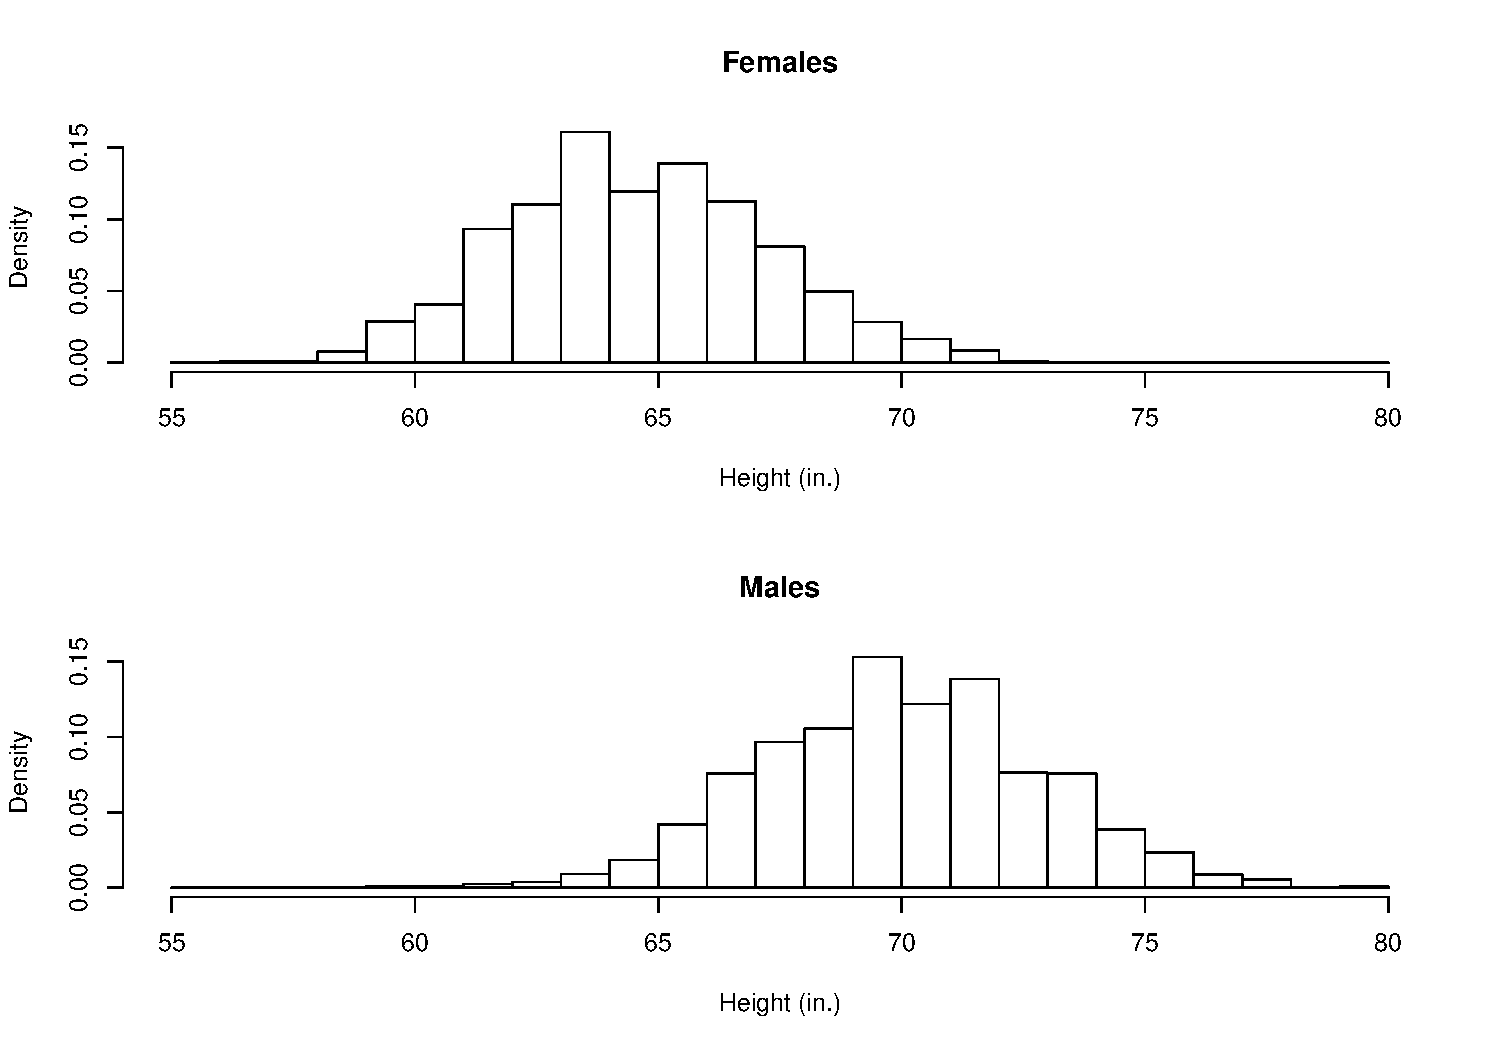
\includegraphics[width=\maxwidth]{figure/heights_by_sex-1} 

}

\caption[Histograms of User Heights Split by Sex]{Histograms of User Heights Split by Sex}\label{fig:heights_by_sex}
\end{figure}


\end{knitrout}


\subsubsection{Pedagogical Discussion}
This first exercise stresses many important considerations students should keep in mind when working with real data.  Firstly, it emphasizes the importance of performing an exploratory data analysis to identify anomalous observations and confronts students with the question of what to do with them.  For example, while a height of 1 inch is clearly an outlier that needs to be removed an instructor can ask at what point does a height no longer become reasonable and what impact does their removal have on their removal?

Secondly, this exercise demonstrates the power of a simple data visualization and hence emphasizes the importance of putting careful thought into their construction.  The better the construction, the better the conveying of the insight.  In our case, while having students plot two histograms simultaneously on the same scale to demonstrate that males have on average greater height may seem to be a rather pedantic goal, we encouraged students to take a closer look at the histograms and steered their focus towards the unusual peaks at 72 inches (6 feet) for males and 64 inches (5'4'') for females.  Many of the students could easily explain the phenomena of the peak at 72 inches for men: sociological perceptions of the rounded height of 6 feet.  On the other hand, consensus was not as strong about perceptions of the height of 5'4'' for women.  Instructors can then refer students to the entry on OkCupid's blog OkTrends ``The Biggest Lies in Online Data''\cite{OkTrendsLies} to show they've replicated (on a smaller scale) a previous analysis done by OkCupid and then show the other examples of analysis of the blog.

Further questions that can be pursued from this exercise include ``How can we question if those peaks are significant or due to chance?'', ``Are we only observing men who are just under 6 feet rounding up, or are men just over 6 feet rounding down as well?'', or ``How can we compare the distribution of listed heights on OkCupid to the actual San Francisco's population height distribution?''







%---------------------------------------------------------------
\subsection{Relationship Between Sex and Sexual Orientation}
%---------------------------------------------------------------
\subsubsection{Exercise}
Since among the most important considerations in assessing a potential mate are their sex and sexual orientation, in this exercise we investigate the relationship between these two variables.  First, we perform a basic exploratory data analysis on these variables using barcharts in Figure \ref{fig:sex_and_orientation} using the code below:

\begin{knitrout}
\definecolor{shadecolor}{rgb}{0.969, 0.969, 0.969}\color{fgcolor}\begin{kframe}
\begin{alltt}
\hlkwd{par}\hlstd{(}\hlkwc{mfrow}\hlstd{=}\hlkwd{c}\hlstd{(}\hlnum{1}\hlstd{,} \hlnum{2}\hlstd{))}
\hlkwd{barplot}\hlstd{(}\hlkwd{table}\hlstd{(profiles}\hlopt{$}\hlstd{sex)}\hlopt{/}\hlstd{n,} \hlkwc{xlab}\hlstd{=}\hlstr{"sex"}\hlstd{,} \hlkwc{ylab}\hlstd{=}\hlstr{"proportion"}\hlstd{)}
\hlkwd{barplot}\hlstd{(}\hlkwd{table}\hlstd{(profiles}\hlopt{$}\hlstd{orientation)}\hlopt{/}\hlstd{n,} \hlkwc{xlab}\hlstd{=}\hlstr{"orientation"}\hlstd{,} \hlkwc{ylab}\hlstd{=}\hlstr{"proportion"}\hlstd{)}
\end{alltt}
\end{kframe}\begin{figure}

{\centering 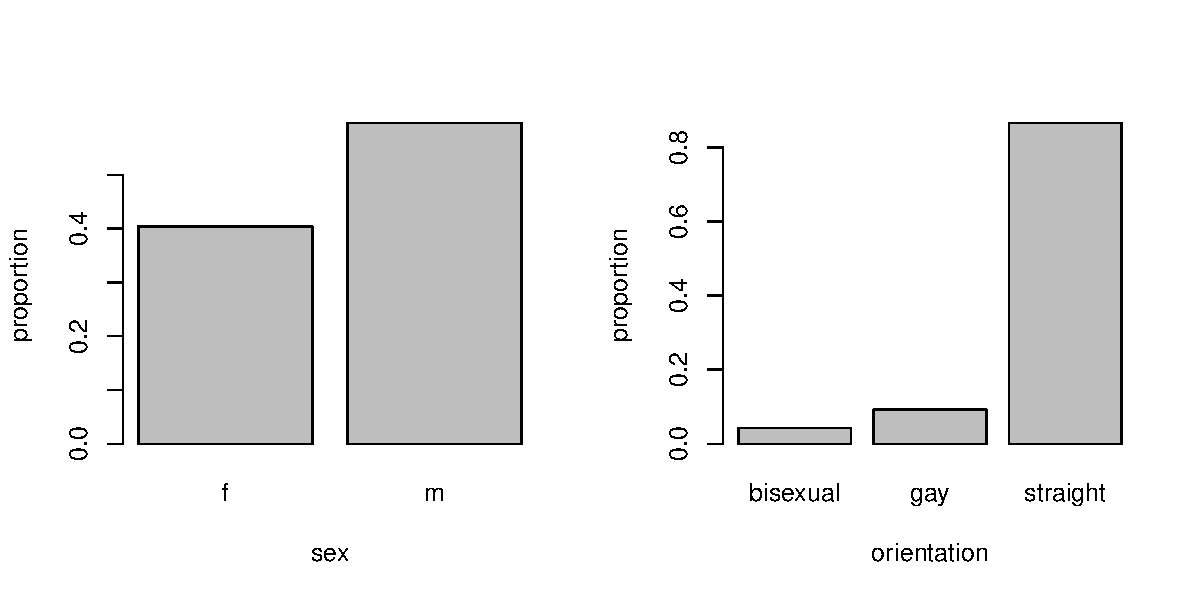
\includegraphics[width=\maxwidth]{figure/sex_and_orientation-1} 

}

\caption[Distributions of Sex and Sexual Orientation]{Distributions of Sex and Sexual Orientation.}\label{fig:sex_and_orientation}
\end{figure}


\end{knitrout}

However, when it comes to dating we can't just consider the \textbf{marginal distributions} (i.e. the margins of a table) of these variables, we must consider their cross-classification i.e. their \textbf{joint distribution}, and \textbf{conditional}.  Only then will we have a more accurate picture of the dating landscape.  We describe the distribution of ``sexual orientation'' conditional on ``sex.''  For example, of all females (the condition) what proportion are bisexual?  We do this using the \verb#tally()# command from the \verb#mosaic# package and visualize this breakdown via a mosaicplot (as shown in Figure \ref{fig:sex_by_orientation}).

\begin{knitrout}
\definecolor{shadecolor}{rgb}{0.969, 0.969, 0.969}\color{fgcolor}\begin{kframe}
\begin{alltt}
\hlkwd{tally}\hlstd{(orientation} \hlopt{~} \hlstd{sex, profiles,} \hlkwc{format}\hlstd{=}\hlstr{'proportion'}\hlstd{)}
\end{alltt}
\begin{verbatim}
##            sex
## orientation     f     m
##    bisexual 0.078 0.018
##    gay      0.065 0.110
##    straight 0.857 0.871
\end{verbatim}
\begin{alltt}
\hlstd{sex.by.orientation} \hlkwb{<-} \hlkwd{with}\hlstd{(profiles,} \hlkwd{table}\hlstd{(sex, orientation))}
\hlkwd{mosaicplot}\hlstd{(sex.by.orientation}\hlopt{/}\hlstd{n,} \hlkwc{main}\hlstd{=}\hlstr{"Sex vs Orientation"}\hlstd{)}
\end{alltt}
\end{kframe}\begin{figure}

{\centering 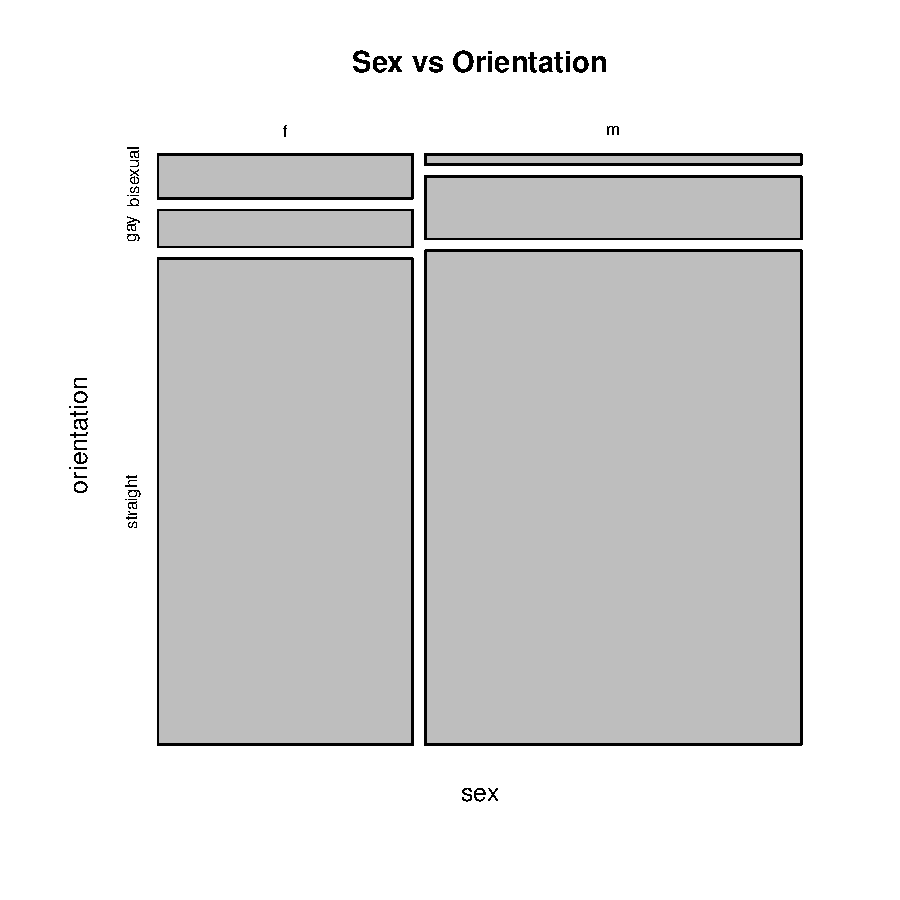
\includegraphics[width=\maxwidth]{figure/sex_by_orientation-1} 

}

\caption[Cross-classification of sex and sexual orientation]{Cross-classification of sex and sexual orientation.}\label{fig:sex_by_orientation}
\end{figure}


\end{knitrout}

We now proceed with the \textit{chi-square tests for independence} to perform one using the \verb#chisq.test()# command.
\begin{knitrout}
\definecolor{shadecolor}{rgb}{0.969, 0.969, 0.969}\color{fgcolor}\begin{kframe}
\begin{alltt}
\hlkwd{chisq.test}\hlstd{(sex.by.orientation)}
\end{alltt}
\begin{verbatim}
## 
## 	Pearson's Chi-squared test
## 
## data:  sex.by.orientation
## X-squared = 154, df = 2, p-value < 2.2e-16
\end{verbatim}
\end{kframe}
\end{knitrout}



\subsubsection{Pedagogical Discussion}
This exercise was an opportunity to concretize the statistical notions such as marginal / joint / conditional distribtions, sampling bias, and ``big data.''

he data indicate that the San Francisco OkCupid dating population skews male and while the proportions of males and females who list themselves as straight are similar, a higher proportion of males list themselves as gay while a higher proportion of females list themselves as bisexual.  Many students were not surprised by this fact as they are well aware of the gender imbalance issues in the Technology sector, the rise of the San Francisco Bay Area as a formidabe tech capitol, and San Francisco's history of being a bastion community for gay men in the recent past.  An interesting discussion arose on the sociological factors in why more women listed themselves as bisexual then men; this topic has previously been covered on the blog OkTrends\cite{OkTrendsLies}.

Students could make statement that are conditional probability statements such as ``Of the female population, $X$\% were $Y$'s and some could even recognize the etiomogical origins of the term "marginal distribution" as their counts are presented in the margins of the table.

The question of generalizability was presented in an introductory probability and statistics class homework.  Almost all students were able to recognize the non-randomness of the sampling and hence the results are non-generalizable.  For example they recognized that OkCupid's demographic is most likely different than other demographics, such as match.com (which is not free) or christiansingles.com (which is targeted towards Christians), or less technology-savvy individuals.

So while 59946 users may seem like a fairly large sample to many students, we emphasized that one must be wary of self-selection biases that can affect the generalizability of the results.  This proved an excellent segue to discussions on John Tukey's famous quote to the sexologist Alfred Kinsey ``A random selection of three people would have been better than a group of 300 chosen by Mr. Kinsey.'' and Kate Crawford of Microsoft Research's YouTube talk ``Algorithmic Illusions: Hidden Biases of Big Data''~\cite{Strata}.

Further questions one can pose to students include ``Which dating demographic would you say has it the best and worst in terms of our simplied categorization?'', ``What variable do you think should be incorporated next after sex and sexual orientation in faithfully representing the OkCupid landscape?'', ``Are we sure we can't \textit{pratically} assume generalizability of the results to Brooklyn OkCupid?''.







%---------------------------------------------------------------
\subsection{Text Analysis}\label{essays}
%---------------------------------------------------------------
\subsubsection{Exercise}

The next exercise focuses on the responses to the essay questions, providing you with an opportunity to perform text analysis.  Manipulating text data in R is often a complicated affair, so we present some code you should not worry if it doesn't make sense at first, as it is for more skilled coders.  The following code
\begin{itemize}
\item Uses the \verb#select()# command from the \verb#dplyr# package to select the 10 essay columms as identified by the fact they \verb#starts_with("essay")#.
\item Converts the essays from list to matrix format.
\item For each user concatenates the 10 columns to form a single string.  The code applies the function \verb#paste(x, collapse=" ")# to every essay where \verb#x# is the set of 10 essay responses, and the \verb#paste()# function collapses \verb#x# across columns while separate the elements by a space.  We do this for each set of essays (i.e. each row of \verb#essays#) via the \verb#apply()# command and setting the second argument to \verb#1#.
\item Replace all line breaks (\verb#\n#) and paragraph breaks (\verb#<br />#) with spaces as well to make the outputs more readable.
\end{itemize}

The output is a single vector \verb#essays# that contains all 10 essay responses for each user concatenated together.

\begin{knitrout}
\definecolor{shadecolor}{rgb}{0.969, 0.969, 0.969}\color{fgcolor}\begin{kframe}
\begin{alltt}
\hlstd{essays} \hlkwb{<-} \hlkwd{select}\hlstd{(profiles,} \hlkwd{starts_with}\hlstd{(}\hlstr{"essay"}\hlstd{))}
\hlstd{essays} \hlkwb{<-} \hlkwd{matrix}\hlstd{(}\hlkwd{unlist}\hlstd{(essays),} \hlkwc{ncol} \hlstd{=} \hlkwd{ncol}\hlstd{(essays),} \hlkwc{byrow} \hlstd{=} \hlnum{FALSE}\hlstd{)}
\hlstd{essays} \hlkwb{<-} \hlkwd{apply}\hlstd{(essays,} \hlnum{1}\hlstd{, paste,} \hlkwc{collapse}\hlstd{=}\hlstr{" "}\hlstd{)}
\hlstd{essays} \hlkwb{<-} \hlkwd{str_replace_all}\hlstd{(essays,} \hlstr{"\textbackslash{}n"}\hlstd{,} \hlstr{" "}\hlstd{)}
\hlstd{essays} \hlkwb{<-} \hlkwd{str_replace_all}\hlstd{(essays,} \hlstr{"<br />"}\hlstd{,} \hlstr{" "}\hlstd{)}
\end{alltt}
\end{kframe}
\end{knitrout}

We ask:  Do men and women OkCupid users use words at different rates in their essay responses?  We can do this using the \verb#str_detect()# command in the \verb#stringr# package to search essays for the word in quotation marks and the \verb#tally()# command from the \verb#mosaic# package to compute the conditional (on sex) distributions.  For example, the word ``book'':

\begin{knitrout}
\definecolor{shadecolor}{rgb}{0.969, 0.969, 0.969}\color{fgcolor}\begin{kframe}
\begin{alltt}
\hlstd{profiles}\hlopt{$}\hlstd{has.book} \hlkwb{<-} \hlkwd{str_detect}\hlstd{(essays,} \hlstr{"book"}\hlstd{)}
\hlkwd{tally}\hlstd{(has.book} \hlopt{~} \hlstd{sex, profiles,} \hlkwc{format}\hlstd{=}\hlstr{'proportion'}\hlstd{)}
\end{alltt}
\begin{verbatim}
##         sex
## has.book    f    m
##    TRUE  0.62 0.55
##    FALSE 0.38 0.45
\end{verbatim}
\end{kframe}
\end{knitrout}

We test out various preconceptions of word use between any of the categorical variables:  sex, sexual orientation, etc.  For example, in Table \ref{word_use_by_sex} we compare the proportion of use of words in essays split by sex.

% latex table generated in R 3.1.2 by xtable 1.7-4 package
% Fri Mar 27 16:16:58 2015
\begin{table}[ht]
\centering
\begin{tabular}{lrr}
  \hline
query & female & male \\ 
  \hline
travel & 0.387 & 0.293 \\ 
  food & 0.655 & 0.602 \\ 
  wine & 0.195 & 0.116 \\ 
  beer & 0.088 & 0.105 \\ 
   \hline
\end{tabular}
\caption{Proportion of use of words in essays split by sex.} 
\label{word_use}
\end{table}


We also verify the co-occurence of words:

\begin{knitrout}
\definecolor{shadecolor}{rgb}{0.969, 0.969, 0.969}\color{fgcolor}\begin{kframe}
\begin{alltt}
\hlstd{profiles}\hlopt{$}\hlstd{has.wine} \hlkwb{<-} \hlkwd{str_detect}\hlstd{(essays,} \hlstr{"wine"}\hlstd{)}
\hlstd{profiles}\hlopt{$}\hlstd{has.travel} \hlkwb{<-} \hlkwd{str_detect}\hlstd{(essays,} \hlstr{"travel"}\hlstd{)}
\hlkwd{tally}\hlstd{(}\hlopt{~}\hlstd{has.travel} \hlopt{+} \hlstd{has.wine,} \hlkwc{data}\hlstd{=profiles)}
\end{alltt}
\begin{verbatim}
##           has.wine
## has.travel TRUE FALSE
##      TRUE   461  1522
##      FALSE  423  3589
\end{verbatim}
\begin{alltt}
\hlkwd{mosaicplot}\hlstd{(}\hlkwd{tally}\hlstd{(}\hlopt{~}\hlstd{has.travel} \hlopt{+} \hlstd{has.wine,} \hlkwc{data}\hlstd{=profiles),} \hlkwc{main}\hlstd{=}\hlstr{""}\hlstd{,} \hlkwc{xlab}\hlstd{=}\hlstr{"Travel"}\hlstd{,}
           \hlkwc{ylab}\hlstd{=}\hlstr{"Wine"}\hlstd{)}
\end{alltt}
\end{kframe}\begin{figure}

{\centering 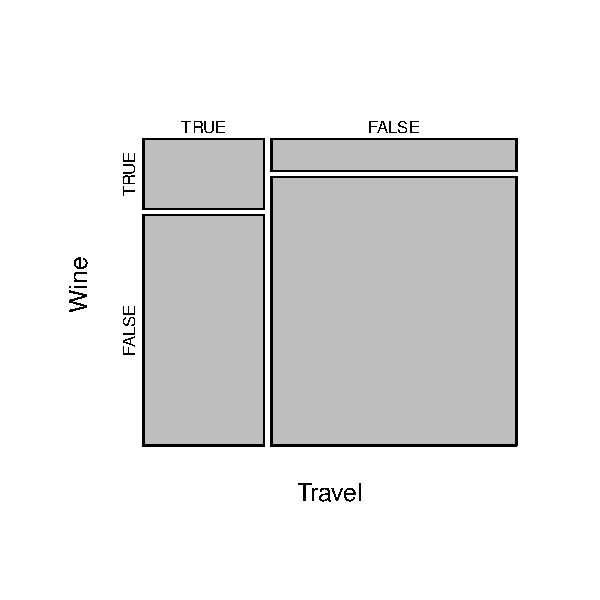
\includegraphics[width=\maxwidth]{figure/travel_vs_wine-1} 

}

\caption[Co-occurrence of 'Travel' and 'Wine']{Co-occurrence of 'Travel' and 'Wine'}\label{fig:travel_vs_wine}
\end{figure}


\end{knitrout}

And finally we evaluate the statistical significance of the difference in the use of the word ``football'' via a two-sample proportions test using the \verb#prop.test()# function where you specify \verb#x# the successes of each group and \verb#n# the numbers in each group.  While the difference of around 0.5\% is statistically significant for almost any $\alpha$-level, it could be argued that this difference is of little practical significance.

\begin{knitrout}
\definecolor{shadecolor}{rgb}{0.969, 0.969, 0.969}\color{fgcolor}\begin{kframe}
\begin{alltt}
\hlstd{profiles}\hlopt{$}\hlstd{has.football} \hlkwb{<-} \hlkwd{str_detect}\hlstd{(essays,} \hlstr{"football"}\hlstd{)}
\hlstd{results} \hlkwb{<-} \hlkwd{table}\hlstd{(profiles}\hlopt{$}\hlstd{has.football, profiles}\hlopt{$}\hlstd{sex)}
\hlkwd{prop.test}\hlstd{(}\hlkwc{x}\hlstd{=results[}\hlnum{2}\hlstd{, ],} \hlkwc{n}\hlstd{=}\hlkwd{colSums}\hlstd{(results),} \hlkwc{alternative}\hlstd{=}\hlstr{"two.sided"}\hlstd{)}
\end{alltt}
\begin{verbatim}
## 
## 	2-sample test for equality of proportions with continuity
## 	correction
## 
## data:  x and n
## X-squared = 2, df = 1, p-value = 0.1546
## alternative hypothesis: two.sided
## 95 percent confidence interval:
##  -0.0166  0.0024
## sample estimates:
## prop 1 prop 2 
##  0.030  0.037
\end{verbatim}
\end{kframe}
\end{knitrout}

And finally, consider the following fun exercise: the words in the male's top 500 that weren't in the women's top 500 and vice-versa.

\begin{knitrout}
\definecolor{shadecolor}{rgb}{0.969, 0.969, 0.969}\color{fgcolor}\begin{kframe}
\begin{alltt}
\hlstd{male.words} \hlkwb{<-} \hlkwd{str_split}\hlstd{(essays[profiles}\hlopt{$}\hlstd{sex} \hlopt{==}\hlstr{"m"}\hlstd{],} \hlstr{" "}\hlstd{)} \hlopt \hlkwd{unlist}\hlstd{()} \hlopt \hlkwd{table}\hlstd{()} \hlopt
  \hlkwd{sort}\hlstd{(}\hlkwc{decreasing}\hlstd{=}\hlnum{TRUE}\hlstd{)} \hlopt \hlkwd{names}\hlstd{()}
\hlstd{female.words} \hlkwb{<-} \hlkwd{str_split}\hlstd{(essays[profiles}\hlopt{$}\hlstd{sex} \hlopt{==}\hlstr{"f"}\hlstd{],} \hlstr{" "}\hlstd{)} \hlopt \hlkwd{unlist}\hlstd{()} \hlopt \hlkwd{table}\hlstd{()} \hlopt
  \hlkwd{sort}\hlstd{(}\hlkwc{decreasing}\hlstd{=}\hlnum{TRUE}\hlstd{)} \hlopt \hlkwd{names}\hlstd{()}
\hlcom{# Words in the males top 500 that weren't in the women's top 500}
\hlkwd{setdiff}\hlstd{(male.words[}\hlnum{1}\hlopt{:}\hlnum{500}\hlstd{], female.words[}\hlnum{1}\hlopt{:}\hlnum{500}\hlstd{])}
\end{alltt}
\begin{verbatim}
##  [1] "words"    "his"      "company"  ","        "video"    "sports"  
##  [7] "else"     "computer" "/"        "john"     "future"   "world."  
## [13] "internet" "well,"    "run"      "three"    "bar"      "work."   
## [19] "short"    "away"     "business" "until"    "side"     "us"      
## [25] "found"    "went"     "science"  "type"     "here."    "isn't"   
## [31] "started"  "stuff."   "career"   "well."    "more."    "show,"   
## [37] "serious"  "star"     "said"     "to."      "women"    "couple"
\end{verbatim}
\begin{alltt}
\hlcom{# Words in the male top 500 that weren't in the women's top 500}
\hlkwd{setdiff}\hlstd{(female.words[}\hlnum{1}\hlopt{:}\hlnum{500}\hlstd{], male.words[}\hlnum{1}\hlopt{:}\hlnum{500}\hlstd{])}
\end{alltt}
\begin{verbatim}
##  [1] "loving"     "hair"       "dog"        "seeing"     "dancing,"  
##  [6] ";)"         "appreciate" "kinds"      "laughing"   "red"       
## [11] "passionate" "hate"       "laugh."     "love,"      "beautiful" 
## [16] "kids"       "david"      "she"        "please"     "crazy"     
## [21] "change"     "2"          "laugh,"     "hiking,"    "smile."    
## [26] "men"        "adventure"  "except"     "sex"        "met"       
## [31] "passion"    "willing"    "does"       "become"     "local"     
## [36] "nature"     "healthy"    "myself."    "you'll"     "beach"     
## [41] "dating"     "human"
\end{verbatim}
\end{kframe}
\end{knitrout}





\subsubsection{Teaching Goals and Discussions}
This exercise provides students with experience performing basic text processing, mining, and analysis.  The messiness of the data is once against exemplified by the precense of HTML tags in the text data.  This messiness is both liability, as only students who are somewhat familiar with R will feel comfortable, as it is asset, as it confronts students with the fact that data-cleaning is a large part of the work.

The nature of the data allows for students to judge prior sociological beliefs and preconceptions using data.  Many students were confronted, even with these simple analyses, with the fact that there is still evident gendered language being used in profile essays, and further investigation is warranted.

Statistical concepts include the difference between practical and statistical significance as demonstrated by the difference in proportion of males and females that used the word ``football''.  This can lead to discussions of what it means to conduct hypothesis tests when the sample size is as large as 59946.  Why it was important to show which words were being used by men \textit{but not by women} as individually both groups will have as most frequently used words that are mostly particles like "the", "and", and "or".

Further avenues of inquest include asking ``What are the implications of performing a large number of these proportions test on the essays?'', ``Can we predict demographic attributes of users based on word use?''  ``For what words do we see the biggest differences in use between the three categories of sexual orientation?''.  An even bolder goal include introducing concepts, such as constructing wordclouds,  inverse document frequency, natural language processing, and Latent dirichlet analysis\cite{LDA:2003}.







%---------------------------------------------------------------
\subsection{Predictors of Sex}
%---------------------------------------------------------------
The final exercise provides an opportunity to fit a predicitive model for sex using logistic regression.  In order to reinforce the concepts of logistic regression, we only consider using one predictor variable in the logistic model: height.  Given our observations in Section \ref{section_height}, we restrict to only those users whose heights are ``reasonable''.

\begin{knitrout}
\definecolor{shadecolor}{rgb}{0.969, 0.969, 0.969}\color{fgcolor}\begin{kframe}
\begin{alltt}
\hlstd{profiles} \hlkwb{<-} \hlkwd{filter}\hlstd{(profiles, height}\hlopt{>=}\hlnum{55} \hlopt{&} \hlstd{height} \hlopt{<=}\hlnum{80}\hlstd{)}
\hlstd{profiles} \hlkwb{<-} \hlkwd{sample_n}\hlstd{(profiles, n}\hlopt{*}\hlnum{0.1}\hlstd{)}
\end{alltt}


{\ttfamily\noindent\bfseries\color{errorcolor}{\#\# Error: Sample size (5994.6) greater than population size (5983). Do you want replace = TRUE?}}\end{kframe}
\end{knitrout}

\subsubsection{Exercise}
We convert the \verb#sex# variable to a binary \verb#is.female# variable, where \verb#1# if female and \verb#0# if male, using the \verb#ifelse()# function.  We plot the points as in Figure \ref{is_female_vs_height}, making use of the \verb#ggplot2# package.

\begin{knitrout}
\definecolor{shadecolor}{rgb}{0.969, 0.969, 0.969}\color{fgcolor}\begin{kframe}
\begin{alltt}
\hlstd{profiles}\hlopt{$}\hlstd{is.female} \hlkwb{=} \hlkwd{ifelse}\hlstd{(profiles}\hlopt{$}\hlstd{sex}\hlopt{==}\hlstr{"f"}\hlstd{,} \hlnum{1}\hlstd{,} \hlnum{0}\hlstd{)}
\hlkwd{ggplot}\hlstd{(}\hlkwc{data}\hlstd{=profiles,} \hlkwd{aes}\hlstd{(}\hlkwc{x}\hlstd{=height,} \hlkwc{y}\hlstd{=is.female))} \hlopt{+} \hlkwd{geom_point}\hlstd{()} \hlopt{+}
  \hlkwd{xlab}\hlstd{(}\hlstr{"Height (in.)"}\hlstd{)} \hlopt{+} \hlkwd{ylab}\hlstd{(}\hlstr{"Is female?"}\hlstd{)}
\end{alltt}
\end{kframe}\begin{figure}

{\centering 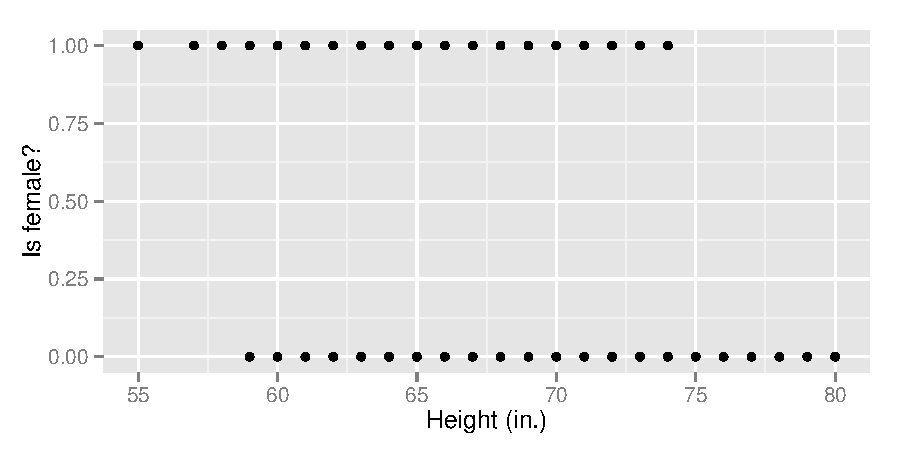
\includegraphics[width=\maxwidth]{figure/is_female_vs_height-1} 

}

\caption[Female Indicator vs Height]{Female Indicator vs Height}\label{fig:is_female_vs_height}
\end{figure}


\end{knitrout}

We question the usefulness of this plot, as the overlap of the points makes it difficult for determine how many points are involved.  We use the \verb#jitter()# function to add a little random noise to each clump of points as shown in Figure \ref{is_female_vs_height_jittered}.

\begin{knitrout}
\definecolor{shadecolor}{rgb}{0.969, 0.969, 0.969}\color{fgcolor}\begin{kframe}
\begin{alltt}
\hlkwd{ggplot}\hlstd{(}\hlkwc{data}\hlstd{=profiles,} \hlkwd{aes}\hlstd{(}\hlkwc{x}\hlstd{=}\hlkwd{jitter}\hlstd{(height),} \hlkwc{y}\hlstd{=}\hlkwd{jitter}\hlstd{(is.female)))} \hlopt{+}
  \hlkwd{geom_point}\hlstd{()} \hlopt{+} \hlkwd{xlab}\hlstd{(}\hlstr{"Height (in.)"}\hlstd{)} \hlopt{+} \hlkwd{ylab}\hlstd{(}\hlstr{"Is female?"}\hlstd{)}
\end{alltt}
\end{kframe}\begin{figure}

{\centering 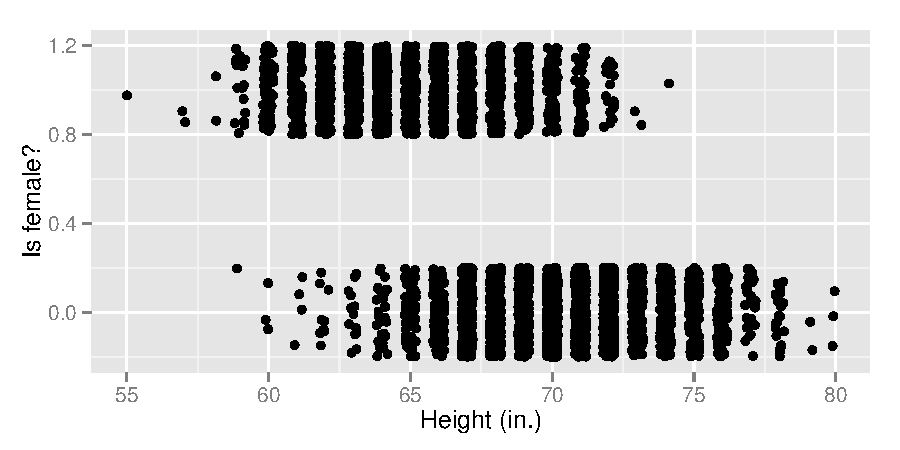
\includegraphics[width=\maxwidth]{figure/is_female_vs_height_jitered-1} 

}

\caption[Female Indicator vs Height]{Female Indicator vs Height}\label{fig:is_female_vs_height_jitered}
\end{figure}


\end{knitrout}

We fit both linear and logistic regression models using height as the sole predictor.  Furthermore, we use the \verb#msummary()# from the \verb#mosaic# command to obtain the regression summary as its output is much more digestible than the output of the \verb#summary()# command.  Furthermore, we extract the coefficients of the linear model using the \verb#coef()# command.

\begin{knitrout}
\definecolor{shadecolor}{rgb}{0.969, 0.969, 0.969}\color{fgcolor}\begin{kframe}
\begin{alltt}
\hlstd{linear.model} \hlkwb{<-} \hlkwd{lm}\hlstd{(is.female} \hlopt{~} \hlstd{height,} \hlkwc{data}\hlstd{=profiles)}
\hlkwd{msummary}\hlstd{(linear.model)}
\end{alltt}
\begin{verbatim}
##             Estimate Std. Error t value Pr(>|t|)    
## (Intercept)   6.3836     0.0819    77.9   <2e-16 ***
## height       -0.0876     0.0012   -73.1   <2e-16 ***
## 
## Residual standard error: 0.36 on 5982 degrees of freedom
## Multiple R-squared:  0.472,	Adjusted R-squared:  0.472 
## F-statistic: 5.34e+03 on 1 and 5982 DF,  p-value: <2e-16
\end{verbatim}
\begin{alltt}
\hlstd{b1} \hlkwb{<-} \hlkwd{coef}\hlstd{(linear.model)}
\end{alltt}
\end{kframe}
\end{knitrout}

\begin{knitrout}
\definecolor{shadecolor}{rgb}{0.969, 0.969, 0.969}\color{fgcolor}\begin{kframe}
\begin{alltt}
\hlstd{logistic.model} \hlkwb{<-} \hlkwd{glm}\hlstd{(is.female} \hlopt{~} \hlstd{height,} \hlkwc{family}\hlstd{=binomial,} \hlkwc{data}\hlstd{=profiles)}
\hlkwd{msummary}\hlstd{(logistic.model)}
\end{alltt}
\begin{verbatim}
## Coefficients:
##             Estimate Std. Error z value Pr(>|z|)    
## (Intercept)  45.5213     1.1566    39.4   <2e-16 ***
## height       -0.6778     0.0171   -39.6   <2e-16 ***
## 
## (Dispersion parameter for binomial family taken to be 1)
## 
##     Null deviance: 8075.5  on 5983  degrees of freedom
## Residual deviance: 4381.5  on 5982  degrees of freedom
## AIC: 4386
## 
## Number of Fisher Scoring iterations: 6
\end{verbatim}
\begin{alltt}
\hlstd{b2} \hlkwb{<-} \hlkwd{coefficients}\hlstd{(logistic.model)}
\end{alltt}
\end{kframe}
\end{knitrout}

In both cases we observe that the coefficient associated with height is negative, in other words, as height increases, the fitted probability of being female decreases.  However the interpretability of the logistic model is difficult.  We thus plot both regressions lines, with the linear regression in red and the logistic regression in blue.  The latter necessitates a function for the inverse logit of the linear equation to obtain:

\[
\widehat{p}_i = \frac{1}{1+\exp\left(-(\widehat{\beta}_0 + \widehat{\beta}_1 \times \mbox{height}_i)\right)}
\]


\begin{knitrout}
\definecolor{shadecolor}{rgb}{0.969, 0.969, 0.969}\color{fgcolor}\begin{kframe}
\begin{alltt}
\hlstd{inverse.logit} \hlkwb{<-} \hlkwa{function}\hlstd{(}\hlkwc{x}\hlstd{,} \hlkwc{b}\hlstd{)\{}
  \hlstd{linear.equation} \hlkwb{<-} \hlstd{b[}\hlnum{1}\hlstd{]} \hlopt{+} \hlstd{b[}\hlnum{2}\hlstd{]}\hlopt{*}\hlstd{x}
  \hlnum{1}\hlopt{/}\hlstd{(}\hlnum{1}\hlopt{+}\hlkwd{exp}\hlstd{(}\hlopt{-}\hlstd{linear.equation))}
\hlstd{\}}
\hlkwd{ggplot}\hlstd{(}\hlkwc{data}\hlstd{=profiles,} \hlkwd{aes}\hlstd{(}\hlkwc{x}\hlstd{=}\hlkwd{jitter}\hlstd{(height),} \hlkwc{y}\hlstd{=}\hlkwd{jitter}\hlstd{(is.female)))} \hlopt{+}
  \hlkwd{geom_point}\hlstd{()} \hlopt{+} \hlkwd{xlab}\hlstd{(}\hlstr{"Height (in.)"}\hlstd{)} \hlopt{+} \hlkwd{ylab}\hlstd{(}\hlstr{"Is female?"}\hlstd{)} \hlopt{+}
  \hlkwd{geom_abline}\hlstd{(}\hlkwc{intercept}\hlstd{=b1[}\hlnum{1}\hlstd{],} \hlkwc{slope}\hlstd{=b1[}\hlnum{2}\hlstd{],} \hlkwc{col}\hlstd{=}\hlstr{"red"}\hlstd{,} \hlkwc{size}\hlstd{=}\hlnum{2}\hlstd{)} \hlopt{+}
  \hlkwd{stat_function}\hlstd{(}\hlkwc{fun} \hlstd{= inverse.logit,} \hlkwc{args}\hlstd{=}\hlkwd{list}\hlstd{(}\hlkwc{b}\hlstd{=b2),} \hlkwc{color}\hlstd{=}\hlstr{"blue"}\hlstd{,} \hlkwc{size}\hlstd{=}\hlnum{2}\hlstd{)}
\end{alltt}
\end{kframe}\begin{figure}

{\centering 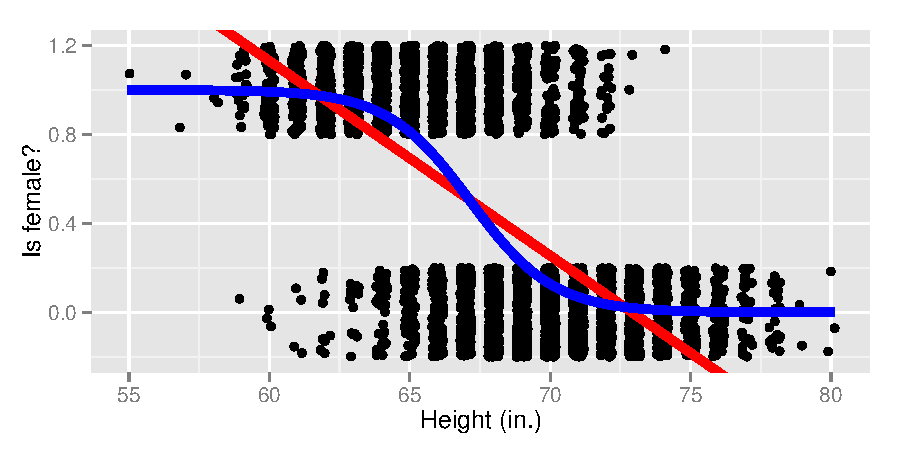
\includegraphics[width=\maxwidth]{figure/is_female_vs_height_3-1} 

}

\caption[Female Indicator vs Height]{Female Indicator vs Height}\label{fig:is_female_vs_height_3}
\end{figure}


\end{knitrout}

We observe that linear regression (red curve) yields fitted probabilities less than 0 for heights less than 61 inches for and fitted probabilities greater than 1 for heights over 73 inches, which do not make sense.  This is not a problem with logistic regression as the inverse-S shaped of the logistic curve ensures fitted probabilities are between 0 and 1 for all heights.   We therefore deem logistic regression to be the appropriate technique for this data.

However, when predicting a user's gender, just using the fitted probabilities $\widehat{p}_i$ are insufficient; a decisions threshold is necessary.  In other words, a point at which if the probability of being a woman is exceeded, we declare that user to be female.

Looking at the histogram of fitted probabilities, we pick an appropriate decision threshold $p^*$ such that for all users who's $\widehat{p}_i > p^*$ we predict the user to be female.  We opt for $p^* = 0.5$ and highlight this in red in Figure \ref{fitted_values}.  In order to evaluate the performance of our model and our decision threshold, we produce the contingency table of the truth and predicted values to evaluate the model performance.

\begin{knitrout}
\definecolor{shadecolor}{rgb}{0.969, 0.969, 0.969}\color{fgcolor}\begin{kframe}
\begin{alltt}
\hlstd{profiles}\hlopt{$}\hlstd{p.hat} \hlkwb{<-} \hlkwd{fitted}\hlstd{(logistic.model)}
\hlkwd{hist}\hlstd{(profiles}\hlopt{$}\hlstd{p.hat,} \hlkwc{xlab}\hlstd{=}\hlstr{"p.hat"}\hlstd{,} \hlkwc{main}\hlstd{=}\hlstr{"Fitted Probabilities of Being Female"}\hlstd{)}
\hlkwd{abline}\hlstd{(}\hlkwc{v}\hlstd{=}\hlnum{0.5}\hlstd{,} \hlkwc{col}\hlstd{=}\hlstr{"red"}\hlstd{,} \hlkwc{lwd}\hlstd{=}\hlnum{2}\hlstd{)}
\end{alltt}
\end{kframe}\begin{figure}

{\centering 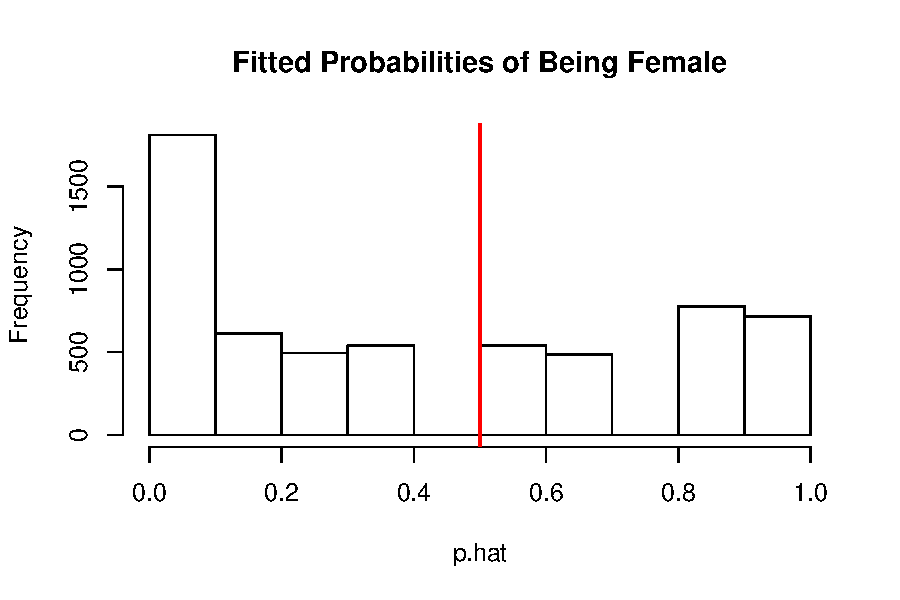
\includegraphics[width=\maxwidth]{figure/fitted_values-1} 

}

\caption[Female Indicator vs Height]{Female Indicator vs Height}\label{fig:fitted_values}
\end{figure}

\begin{kframe}\begin{alltt}
\hlstd{profiles}\hlopt{$}\hlstd{predicted.female} \hlkwb{<-} \hlstd{profiles}\hlopt{$}\hlstd{p.hat} \hlopt{>=} \hlnum{0.5}
\hlkwd{table}\hlstd{(}\hlkwc{truth}\hlstd{=profiles}\hlopt{$}\hlstd{is.female,} \hlkwc{prediction}\hlstd{=profiles}\hlopt{$}\hlstd{predicted.female)}
\end{alltt}
\begin{verbatim}
##      prediction
## truth FALSE TRUE
##     0  3014  550
##     1   449 1971
\end{verbatim}
\end{kframe}
\end{knitrout}



\subsubsection{Pedagogical Discussion}
We find that the jump from linear to logistic regression is really hard for students to grasp.  For example, students often ask ``Why the $\log$ and $\exp$ functions?'', ``So we're not modelling $Y_i$ the outcome variable, we're modeling the probability $p_i$ that it equals 1?'', ``Why does the linear equation model the odds and not $p_i$ or $Y_i$''.  This exercise provides students to build up to the notion of logistic regression from the ground up and using data visualizations.  This example does however require familiarity with the \verb#ggplot2# package.  We feel this is a tool any data scientist primarily using \verb#R# should use, and have incorporated it heavily into our data science class.

We also argue that it is insufficient to merely fit the model and interpret any regressions, we feel that students benefit by also having predictions explicitly made and evaluating the logistic model's predictive power.  Wee ask the students ``For what proportion of people did you guess wrong'' referring to the misclassification error rate, in this case 16.69\%.

Further investigations including more than one predictor?  Perhaps using essay based information like in Section \ref{essays}?  What is our \textit{false positive rate} i.e. the proportion of user's who were predicted to be female who were actually male?  What is our \textit{false negative rate} i.e. the proportion of user's who were predicted to be male who were actually female?  If you wanted to be sure you predicted all women correctly, what decision threshold $p^*$ should you use?












%------------------------------------------------------------------------------
%
\section{Conclusions}
%
%------------------------------------------------------------------------------
We feel that this dataset is an ideal one for introducing students to data science as it is

\begin{enumerate}
\item The data consists of an array of categorial, ordinal, numerical, and text variables.
\item This is an instance of real data that is messy and thus requiring data-wrangling, has many suspicious values, and includes categorical variables of a complicated nature (for instance, there are 218 unique responses to the ethnicity variable).  This reinforces to students that time and energy must be often invested into preparing the data for analysis.
\item The dataset is of modest size.  While $n = 59946$ is not an overwhelmingly large number of observations, it is still much larger than typical datasets used in many introductory probability and statistics classes.
\end{enumerate}

We argue that given the salience of the dataset to students, this dataset provides a very fruitful channel to introduce statistical and data sciences to students of vary undergraduate levels.  By presenting questions to students that allow for the use of background knowledge of the problem, whether it be the news, stereotypes, sociological knowledge, students are much better primed to absorb statistical lessons.  Hence, we took a "lead by the hand" approach to the tone of the exercises.  Other statistics education papers taking a similar approach to ours but using different data include BLAH

The R code used in this \verb#.Rmd# R Sweave document can be outputed into an R script file by using the \verb#purl()# command in the \verb#knitr# package on the \verb#JSE.Rnw# R Sweave document found at \url{https://github.com/rudeboybert/JSE_OkCupid}.
\begin{knitrout}
\definecolor{shadecolor}{rgb}{0.969, 0.969, 0.969}\color{fgcolor}\begin{kframe}
\begin{alltt}
\hlkwd{purl}\hlstd{(}\hlkwc{input}\hlstd{=}\hlstr{"JSE.Rnw"}\hlstd{,} \hlkwc{output}\hlstd{=}\hlstr{"JSE.R"}\hlstd{,} \hlkwc{quiet}\hlstd{=}\hlnum{TRUE}\hlstd{)}
\end{alltt}
\end{kframe}
\end{knitrout}










%------------------------------------------------------------------------------
%
\section{Acknowledgements}\label{ack}
%
%------------------------------------------------------------------------------
First, we thank OkCupid President and co-founder Christian Rudder for agreeing to our use of this dataset (under the condition that the dataset remains public).  Second, we thank Everett Wetchler \href{mailto:everett.wetchler@gmail.com}{everett.wetchler@gmail.com} for providing the data; the python script used to scrape the data and the original CSV file of the data can be found at \href{https://github.com/evee746/okcupid}{https://github.com/evee746/okcupid}.  Finally, we thank the reviewers for their helpful comments.

\noindent\makebox[\linewidth]{\rule{\textwidth}{0.4pt}}

\noindent Albert Y. Kim\\
Mathematics Department\\
Reed College\\
3203 SE Woodstock Blvd\\
Portland, OR 97202\\
\href{mailto:albert.kim@reed.edu}{albert.kim@reed.edu}\\

\noindent Adriana Escobedo-Land\\
Reed College\\
3203 SE Woodstock Blvd\\
Portland, OR 97202\\
\href{mailto:escobad@reed.edu}{escobad@reed.edu}










%------------------------------------------------------------------------------
%
% Bibliography
%
%------------------------------------------------------------------------------
\bibliographystyle{unsrt}
\bibliography{JSE}



\end{document}
